\documentclass[11pt,oneside]{book}

%%%%%%%%%%%%%%%%%%%%%%%%%%%%%%%%%%%%%%%%%%%%%%%%%%%%%%%%%%%%%%%%%%%%%%%%%%%%%%%%%%%%%%%%%%%%%%%%%%%
%                                                                                                 %
% The mathematical style of these documents follows                                               %
%                                                                                                 %
% A. Thompson and B.N. Taylor. The NIST Guide for the Use of the International System of Units.   %
%    NIST Special Publication 881, 2008.                                                          %
%                                                                                                 %
% http://www.nist.gov/pml/pubs/sp811/index.cfm                                                    %
%                                                                                                 %
%%%%%%%%%%%%%%%%%%%%%%%%%%%%%%%%%%%%%%%%%%%%%%%%%%%%%%%%%%%%%%%%%%%%%%%%%%%%%%%%%%%%%%%%%%%%%%%%%%%

% $Date: 2013-11-26 10:43:59 -0500 (Tue, 26 Nov 2013) $
% $Revision: 17538 $
% $Author: gforney $

%%%%%%%%%%%%%%%%%%%%%%%%%%%%%%%%%%%%%%%%%%%%%%%%%%%%%%%%%%%%%%%%%%%%%%%%%%%%%%%%%%%%%%%%%%%%%%%%%%%
%                                                                                                 %
% The mathematical style of these documents follows                                               %
%                                                                                                 %
% A. Thompson and B.N. Taylor. The NIST Guide for the Use of the International System of Units.   %
%    NIST Special Publication 881, 2008.                                                          %
%                                                                                                 %
% http://www.nist.gov/pml/pubs/sp811/index.cfm                                                    %
%                                                                                                 %
%%%%%%%%%%%%%%%%%%%%%%%%%%%%%%%%%%%%%%%%%%%%%%%%%%%%%%%%%%%%%%%%%%%%%%%%%%%%%%%%%%%%%%%%%%%%%%%%%%%

% Packages which force the use of better TeX coding
% Mostly from http://tex.stackexchange.com/q/19264
%%\RequirePackage[l2tabu, orthodox]{nag}
%%\usepackage{fixltx2e}
%\usepackage{isomath} % Disabled for the moment because it changes the syntax for bold and roman Greek math symbols
%%\usepackage[all,warning]{onlyamsmath}
%\usepackage{strict} % Commented out for now because it is uncommon. A copy of style.sty is in Manuals/LaTeX_Style_Files/.

\usepackage{times,mathptmx}
\usepackage[pdftex]{graphicx}
\usepackage{tabularx,ragged2e,booktabs,caption}
\usepackage{multirow}
\usepackage{pdfsync}
\usepackage{tikz}
\usepackage{pgfplots}
%\pgfplotsset{compat=1.7}
\usepackage{tocloft}
\usepackage{color}
\usepackage{amsmath}
\definecolor{linknavy}{rgb}{0,0,0.50196}
\definecolor{linkred}{rgb}{1,0,0}
\definecolor{linkblue}{rgb}{0,0,1}
\usepackage{float}
\usepackage{caption}
\usepackage{graphpap}
\usepackage{rotating}
\usepackage{graphicx}
\usepackage{geometry}
\usepackage{relsize}
\usepackage{longtable}
\usepackage{lscape}
\usepackage{amssymb}
\usepackage{makeidx} % Create index at end of document
\usepackage[nottoc,notlof,notlot]{tocbibind} % Put the bibliography and index in the ToC
\usepackage{lastpage} % Automatic last page number reference.
\usepackage[T1]{fontenc}
\usepackage{enumerate}
\usepackage{upquote}
\usepackage{moreverb}
\usepackage{xfrac}
\usepackage{cite}

\newcommand{\nopart}{\expandafter\def\csname Parent-1\endcsname{}} % To fix table of contents in pdf.
\newcommand{\ct}{\tt\small} % eventually will be deprecated due to http://www.tex.ac.uk/cgi-bin/texfaq2html?label=2letterfontcmd
\newcommand{\textct}[1]{\texttt{\small #1}}

\usepackage{tocstyle} % Fix table of contents sections from overlapping section titles
\usetocstyle{standard}
\usepackage{siunitx}
\sisetup{
    detect-all = true,
    input-decimal-markers = {.},
    input-ignore = {,},
    inter-unit-product = \ensuremath{{}\cdot{}},
    multi-part-units = repeat,
    number-unit-product = \text{~},
    per-mode = fraction,
    separate-uncertainty = true,
}

\usepackage{listings}
\usepackage{textcomp}
\definecolor{lbcolor}{rgb}{0.96,0.96,0.96}
\lstset{
    %backgroundcolor=\color{lbcolor},
    tabsize=4,
    rulecolor=,
    language=Fortran,
        basicstyle=\footnotesize\ttfamily,
        upquote=true,
        aboveskip={\baselineskip},
        belowskip={\baselineskip},
        columns=fixed,
        extendedchars=true,
        breaklines=true,
        breakatwhitespace=true,
        frame=none,
        showtabs=false,
        showspaces=false,
        showstringspaces=false,
        identifierstyle=\ttfamily,
        keywordstyle=\color[rgb]{0,0,0},
        commentstyle=\color[rgb]{0,0,0},
        stringstyle=\color[rgb]{0,0,0},
}

\usepackage[pdftex,
        colorlinks=true,
        urlcolor=linkblue,     % \href{...}{...} external (URL)
        citecolor=linkred,     % citation number colors
        linkcolor=linknavy,    % \ref{...} and \pageref{...}
        pdfproducer={pdflatex},
        pdfpagemode=UseNone,
        bookmarksopen=true,
        plainpages=false,
        verbose]{hyperref}

% The Following commented code makes the ``Draft'' watermark on each page.
%\usepackage{eso-pic}
%\usepackage{type1cm}
%\makeatletter
%   \AddToShipoutPicture{
%     \setlength{\@tempdimb}{.5\paperwidth}
%     \setlength{\@tempdimc}{.5\paperheight}
%     \setlength{\unitlength}{1pt}
%     \put(\strip@pt\@tempdimb,\strip@pt\@tempdimc){
%     \makebox(0,0){\rotatebox{45}{\textcolor[gray]{0.75}{\fontsize{8cm}\selectfont{RC6}}}}}
% }
%\makeatother

\setlength{\textwidth}{6.5in}
\setlength{\textheight}{9.0in}
\setlength{\topmargin}{0.in}
\setlength{\headheight}{0.pt}
\setlength{\headsep}{0.in}
\setlength{\parindent}{0.25in}
\setlength{\oddsidemargin}{0.0in}
\setlength{\evensidemargin}{0.0in}
\setlength{\leftmargini}{\parindent} % Controls the indenting of the "bullets" in a list
\setlength{\cftsecnumwidth}{0.45in}
\setlength{\cftsubsecnumwidth}{0.5in}
\setlength{\cftfignumwidth}{0.45in}
\setlength{\cfttabnumwidth}{0.45in}

\newcommand{\titlesigs}
{
\small
\flushright{U.S. Department of Commerce \\
{\em Penny Pritzker, Secretary} \\
\hspace{1in} \\
National Institute of Standards and Technology \\
{\em Willie May, Under Secretary of Commerce for Standards and Technology and Acting Director} }
}

% commands to use for "official" cover and title pages
% see smokeview verification guide to see how they are used

\newcommand{\headerA}[1]{
\flushright{
\fontsize{20}{24}\selectfont
\bf{NIST Special Publication #1}}
}

\newcommand{\headerB}[1]{
\flushright{
\fontsize{28}{33.6}\selectfont
\bf{#1}
}
}

\newcommand{\headerC}[1]{
\vspace{.5in}
\flushright{\fontsize{14}{16.8}\selectfont
#1}
}

\frenchspacing

\newcommand{\dod}[2]{\frac{\partial #1}{\partial #2}}
\newcommand{\DoD}[2]{\frac{\mathrm{D} #1}{\mathrm{D} #2}}
\newcommand{\dsods}[2]{\frac{\partial^2 #1}{\partial #2^2}}
\renewcommand{\d}{\,\mathrm{d}}
\newcommand{\dx}{\delta x}
\newcommand{\dy}{\delta y}
\newcommand{\dz}{\delta z}
\newcommand{\degF}{$^\circ$F}
\newcommand{\degC}{$^\circ$C}
\newcommand{\x}{x}
\newcommand{\y}{y}
\newcommand{\z}{z}
\newcommand{\dt}{\delta t}
\newcommand{\dn}{\delta n}
\newcommand{\cH}{H}
\newcommand{\hu}{u}
\newcommand{\hv}{v}
\newcommand{\hw}{w}
\newcommand{\la}{\lambda}
\newcommand{\bO}{{\Omega}}
\newcommand{\bo}{{\mathbf{\omega}}}
\newcommand{\btau}{\mathbf{\tau}}
\newcommand{\bdelta}{{\mathbf{\delta}}}
\newcommand{\sumyw}{\sum (Y_\alpha/W_\alpha)}
\newcommand{\oW}{\overline{W}}
\newcommand{\om}{\ensuremath{\omega}}
\newcommand{\omx}{\omega_x}
\newcommand{\omy}{\omega_y}
\newcommand{\omz}{\omega_z}
\newcommand{\erf}{\hbox{erf}}
\newcommand{\erfc}{\hbox{erfc}}
\newcommand{\bF}{{\mathbf{F}}}
\newcommand{\bG}{{\mathbf{G}}}
\newcommand{\bof}{{\mathbf{f}}}
\newcommand{\bq}{{\mathbf{q}}}
\newcommand{\br}{{\mathbf{r}}}
\newcommand{\bu}{{\mathbf{u}}}
\newcommand{\bx}{{\mathbf{x}}}
\newcommand{\bk}{{\mathbf{k}}}
\newcommand{\bv}{{\mathbf{v}}}
\newcommand{\bg}{{\mathbf{g}}}
\newcommand{\bn}{{\mathbf{n}}}
\newcommand{\bS}{{\mathbf{S}}}
\newcommand{\bW}{\overline{W}}
\newcommand{\dS}{d{\mathbf{S}}}
\newcommand{\bs}{{\mathbf{s}}}
\newcommand{\bI}{{\mathbf{I}}}
\newcommand{\hp}{H}
\newcommand{\trho}{\tilde{\rho}}
\newcommand{\dph}{{\delta\phi}}
\newcommand{\dth}{{\delta\theta}}
\newcommand{\tp}{\tilde{p}}
\newcommand{\bp}{\overline{p}}
\newcommand{\dQ}{\dot{Q}}
\newcommand{\dq}{\dot{q}}
\newcommand{\dbq}{\dot{\mathbf{q}}}
\newcommand{\dm}{\dot{m}}
\newcommand{\ha}{\frac{1}{2}}
\newcommand{\ft}{\frac{4}{3}}
\newcommand{\ot}{\frac{1}{3}}
\newcommand{\fofi}{\frac{4}{5}}
\newcommand{\of}{\frac{1}{4}}
\newcommand{\twth}{\frac{2}{3}}
\newcommand{\R}{R}
\newcommand{\be}{\begin{equation}}
\newcommand{\ee}{\end{equation}}
\newcommand{\RE}{\hbox{Re}}
\newcommand{\LE}{\hbox{Le}}
\newcommand{\PR}{\hbox{Pr}}
\newcommand{\PE}{\hbox{Pe}}
\newcommand{\NU}{\hbox{Nu}}
\newcommand{\SC}{\hbox{Sc}}
\newcommand{\SH}{\hbox{Sh}}
\newcommand{\WE}{\hbox{We}}
\newcommand{\COTWO}{\text{\tiny \hbox{CO}$_2$}}
\newcommand{\HTWOO}{\text{\tiny \hbox{H}$_2$\hbox{O}}}
\newcommand{\OTWO}{\text{\tiny \hbox{O}$_2$}}
\newcommand{\NTWO}{\text{\tiny \hbox{N}$_2$}}
\newcommand{\CO}{\text{\tiny \hbox{CO}}}
\newcommand{\F}{\text{\tiny \hbox{F}}}
\newcommand{\C}{\text{\tiny \hbox{C}}}
\newcommand{\Hy}{\text{\tiny \hbox{H}}}
\newcommand{\So}{\text{\tiny \hbox{S}}}
\newcommand{\M}{\text{\tiny \hbox{M}}}
\newcommand{\xx}{\text{\tiny \hbox{x}}}
\newcommand{\yy}{\text{\tiny \hbox{y}}}
\newcommand{\zz}{\text{\tiny \hbox{z}}}
\newcommand{\smvlines}{115~000}

\newcommand{\calH}{\mathcal{H}}
\newcommand{\calR}{\mathcal{R}}

\newcommand{\dif}{\mathrm{d}}
\newcommand{\Div}{\nabla\cdot}
\newcommand{\D}{\mbox{D}}
\newcommand{\mhalf}{\mbox{$\frac{1}{2}$}}
\newcommand{\thalf}{\mbox{\tiny $\frac{1}{2}$}}
\newcommand{\tripleprime}{{\prime\prime\prime}}
\newcommand{\ppp}{{\prime\prime\prime}}
\newcommand{\pp}{{\prime\prime}}

\newcommand{\superscript}[1]{\ensuremath{^{\textrm{\tiny #1}}}}
\newcommand{\subscript}[1]{\ensuremath{_{\textrm{\tiny #1}}}}

\newcommand{\rb}[1]{\raisebox{1.5ex}[0pt]{#1}}

\newcommand{\Ra}{$\Rightarrow$}
\newcommand{\hhref}[1]{\href{#1}{{\tt #1}}}
\newcommand{\fdsinput}[1]{{\scriptsize\verbatiminput{../../Verification/Visualization/#1}}}

\definecolor{AQUAMARINE}{rgb}{0.49804,1.00000,0.83137}
\definecolor{ANTIQUE WHITE}{rgb}{0.98039,0.92157,0.84314}
\definecolor{BEIGE}{rgb}{0.96078,0.96078,0.86275}
\definecolor{BLACK}{rgb}{0.00000,0.00000,0.00000}
\definecolor{BLUE}{rgb}{0.00000,0.00000,1.00000}
\definecolor{BLUE VIOLET}{rgb}{0.54118,0.16863,0.88627}
\definecolor{BRICK}{rgb}{0.61176,0.40000,0.12157}
\definecolor{BROWN}{rgb}{0.64706,0.16471,0.16471}
\definecolor{BURNT SIENNA}{rgb}{0.54118,0.21176,0.05882}
\definecolor{BURNT UMBER}{rgb}{0.54118,0.20000,0.14118}
\definecolor{CADET BLUE}{rgb}{0.37255,0.61961,0.62745}
\definecolor{CHOCOLATE}{rgb}{0.82353,0.41176,0.11765}
\definecolor{COBALT}{rgb}{0.23922,0.34902,0.67059}
\definecolor{CORAL}{rgb}{1.00000,0.49804,0.31373}
\definecolor{CYAN}{rgb}{0.00000,1.00000,1.00000}
\definecolor{DIMGRAY }{rgb}{0.41176,0.41176,0.41176}
\definecolor{EMERALD GREEN}{rgb}{0.00000,0.78824,0.34118}
\definecolor{FIREBRICK}{rgb}{0.69804,0.13333,0.13333}
\definecolor{FLESH}{rgb}{1.00000,0.49020,0.25098}
\definecolor{FOREST GREEN}{rgb}{0.13333,0.54510,0.13333}
\definecolor{GOLD }{rgb}{1.00000,0.84314,0.00000}
\definecolor{GOLDENROD}{rgb}{0.85490,0.64706,0.12549}
\definecolor{GRAY}{rgb}{0.50196,0.50196,0.50196}
\definecolor{GREEN}{rgb}{0.00000,1.00000,0.00000}
\definecolor{GREEN YELLOW}{rgb}{0.67843,1.00000,0.18431}
\definecolor{HONEYDEW}{rgb}{0.94118,1.00000,0.94118}
\definecolor{HOT PINK}{rgb}{1.00000,0.41176,0.70588}
\definecolor{INDIAN RED}{rgb}{0.80392,0.36078,0.36078}
\definecolor{INDIGO}{rgb}{0.29412,0.00000,0.50980}
\definecolor{IVORY}{rgb}{1.00000,1.00000,0.94118}
\definecolor{IVORY BLACK}{rgb}{0.16078,0.14118,0.12941}
\definecolor{KELLY GREEN}{rgb}{0.00000,0.50196,0.00000}
\definecolor{KHAKI}{rgb}{0.94118,0.90196,0.54902}
\definecolor{LAVENDER}{rgb}{0.90196,0.90196,0.98039}
\definecolor{LIME GREEN}{rgb}{0.19608,0.80392,0.19608}
\definecolor{MAGENTA}{rgb}{1.00000,0.00000,1.00000}
\definecolor{MAROON}{rgb}{0.50196,0.00000,0.00000}
\definecolor{MELON}{rgb}{0.89020,0.65882,0.41176}
\definecolor{MIDNIGHT BLUE}{rgb}{0.09804,0.09804,0.43922}
\definecolor{MINT}{rgb}{0.74118,0.98824,0.78824}
\definecolor{NAVY}{rgb}{0.00000,0.00000,0.50196}
\definecolor{OLIVE}{rgb}{0.50196,0.50196,0.00000}
\definecolor{OLIVE DRAB}{rgb}{0.41961,0.55686,0.13725}
\definecolor{ORANGE}{rgb}{1.00000,0.50196,0.00000}
\definecolor{ORANGE RED}{rgb}{1.00000,0.27059,0.00000}
\definecolor{ORCHID}{rgb}{0.85490,0.43922,0.83922}
\definecolor{PINK}{rgb}{1.00000,0.75294,0.79608}
\definecolor{POWDER BLUE}{rgb}{0.69020,0.87843,0.90196}
\definecolor{PURPLE}{rgb}{0.50196,0.00000,0.50196}
\definecolor{RASPBERRY}{rgb}{0.52941,0.14902,0.34118}
\definecolor{RED}{rgb}{1.00000,0.00000,0.00000}
\definecolor{ROYAL BLUE}{rgb}{0.25490,0.41176,0.88235}
\definecolor{SALMON}{rgb}{0.98039,0.50196,0.44706}
\definecolor{SANDY BROWN}{rgb}{0.95686,0.64314,0.37647}
\definecolor{SEA GREEN}{rgb}{0.32941,1.00000,0.62353}
\definecolor{SEPIA}{rgb}{0.36863,0.14902,0.07059}
\definecolor{SIENNA}{rgb}{0.62745,0.32157,0.17647}
\definecolor{SILVER}{rgb}{0.75294,0.75294,0.75294}
\definecolor{SKY BLUE}{rgb}{0.52941,0.80784,0.92157}
\definecolor{SLATEBLUE}{rgb}{0.41569,0.35294,0.80392}
\definecolor{SLATE GRAY}{rgb}{0.43922,0.50196,0.56471}
\definecolor{SPRING GREEN}{rgb}{0.00000,1.00000,0.49804}
\definecolor{STEEL BLUE}{rgb}{0.27451,0.50980,0.70588}
\definecolor{TAN}{rgb}{0.82353,0.70588,0.54902}
\definecolor{TEAL}{rgb}{0.00000,0.50196,0.50196}
\definecolor{THISTLE}{rgb}{0.84706,0.74902,0.84706}
\definecolor{TOMATO }{rgb}{1.00000,0.38824,0.27843}
\definecolor{TURQUOISE}{rgb}{0.25098,0.87843,0.81569}
\definecolor{VIOLET}{rgb}{0.93333,0.50980,0.93333}
\definecolor{VIOLET RED}{rgb}{0.81569,0.12549,0.56471}
\definecolor{WHITE}{rgb}{1.00000,1.00000,1.00000}
\definecolor{YELLOW}{rgb}{1.00000,1.00000,0.00000}

\pgfplotsset{
	colormap={blackwhite}{[5pt]
		rgb255(0pt)=(0,0,255); 
		rgb255(100pt)=(0,255,255); 
		rgb255(200pt)=(0,255,0); 
		rgb255(300pt)=(255,255,0); 
		rgb255(400pt)=(255,0,0)
	},
} % defines smokeview colorbar


\floatstyle{boxed}
\newfloat{notebox}{H}{lon}
\newfloat{warning}{H}{low}

% Set default longtable alignment
\setlength\LTleft{0pt}
\setlength\LTright{0pt}


\renewcommand{\bibname}{Equipment_Guide}

% Math shortcuts
\renewcommand{\sb}[1]{_\mathrm{#1}}
\renewcommand{\C}{\mbox{C}}
\renewcommand{\H}{\mbox{H}}
\renewcommand{\O}{\mbox{O}}
\newcommand{\N}{\mbox{N}}

\begin{document}

\bibliographystyle{unsrt}
\pagestyle{empty}

\begin{minipage}[t][9in][s]{6.25in}

\headerB{
Fire Fighting Technology \\
Equipment and Testing Guide
}

\headerC{
\flushright{
Kristopher J. Overholt \\
Craig G. Weinschenk \\
Roy A. McLane \\
Jay A. McElroy \\
Daniel Madrzykowski \\
\bigskip
{\em Fire Research Division \\
Engineering Laboratory \\
Gaithersburg, Maryland, USA} \\ }
}

\flushright{\today \\
}

\vfill

\flushright{

\includegraphics[width=2.in]{../../Bibliography/nistident_flright_vec} \\[.3in]
}

\titlesigs

\end{minipage}

\newpage

\frontmatter

\pagestyle{plain}
\pagenumbering{roman}

\cleardoublepage
\phantomsection
\addcontentsline{toc}{chapter}{Contents}
\tableofcontents

\cleardoublepage
\phantomsection
\addcontentsline{toc}{chapter}{List of Figures}
\listoffigures

\cleardoublepage
\phantomsection
\addcontentsline{toc}{chapter}{List of Tables}
\listoftables

\chapter{List of Acronyms}

\begin{tabbing}
\hspace{1.5in} \= \\
BDP \> Bi-Directional Probe \\
DVR \> Digital Video Recorder \\
NI \> National Instruments \\
NIST \> National Institute of Standards and Technology \\
TC \> Thermocouple \\
\end{tabbing}

\mainmatter


\chapter{Data Acquisition System}
\label{chap:DAQ}

\section{Hardware}
Data acquisition systems are constructed using National Instruments (NI) hardware. The systems starts with the chassis - NI SCXI-1000/NI SCXI-1001. The 1000 is a 4-slot chassis while the 1001 is a 12-slot chassis. The max scan rate of the chassis is (5~$\mu$s $\times$ \# of channels used)$^{-1}$. A 200~kS/s 16-bit digitizer, NI SCXI-1600, connects the chassis to the computer (via USB). The remaining chassis slots are filled with the NI SCXI-1102. The SCXI-1102 is a 32-channel thermocouple amplifier/voltage input module. Each SCXI-1102 is connected to a TC-2095; a shielded, 32-channel, rack-mountable terminal accessory. All of the measurement devices connect to the TC-2095 using either chromel-alumel connectors (temperature) or copper-copper connectors (voltage). A schematic of the hardware configuration is shown in Fig.~(\ref{fig:daq_schem}).

\begin{figure}[h!]
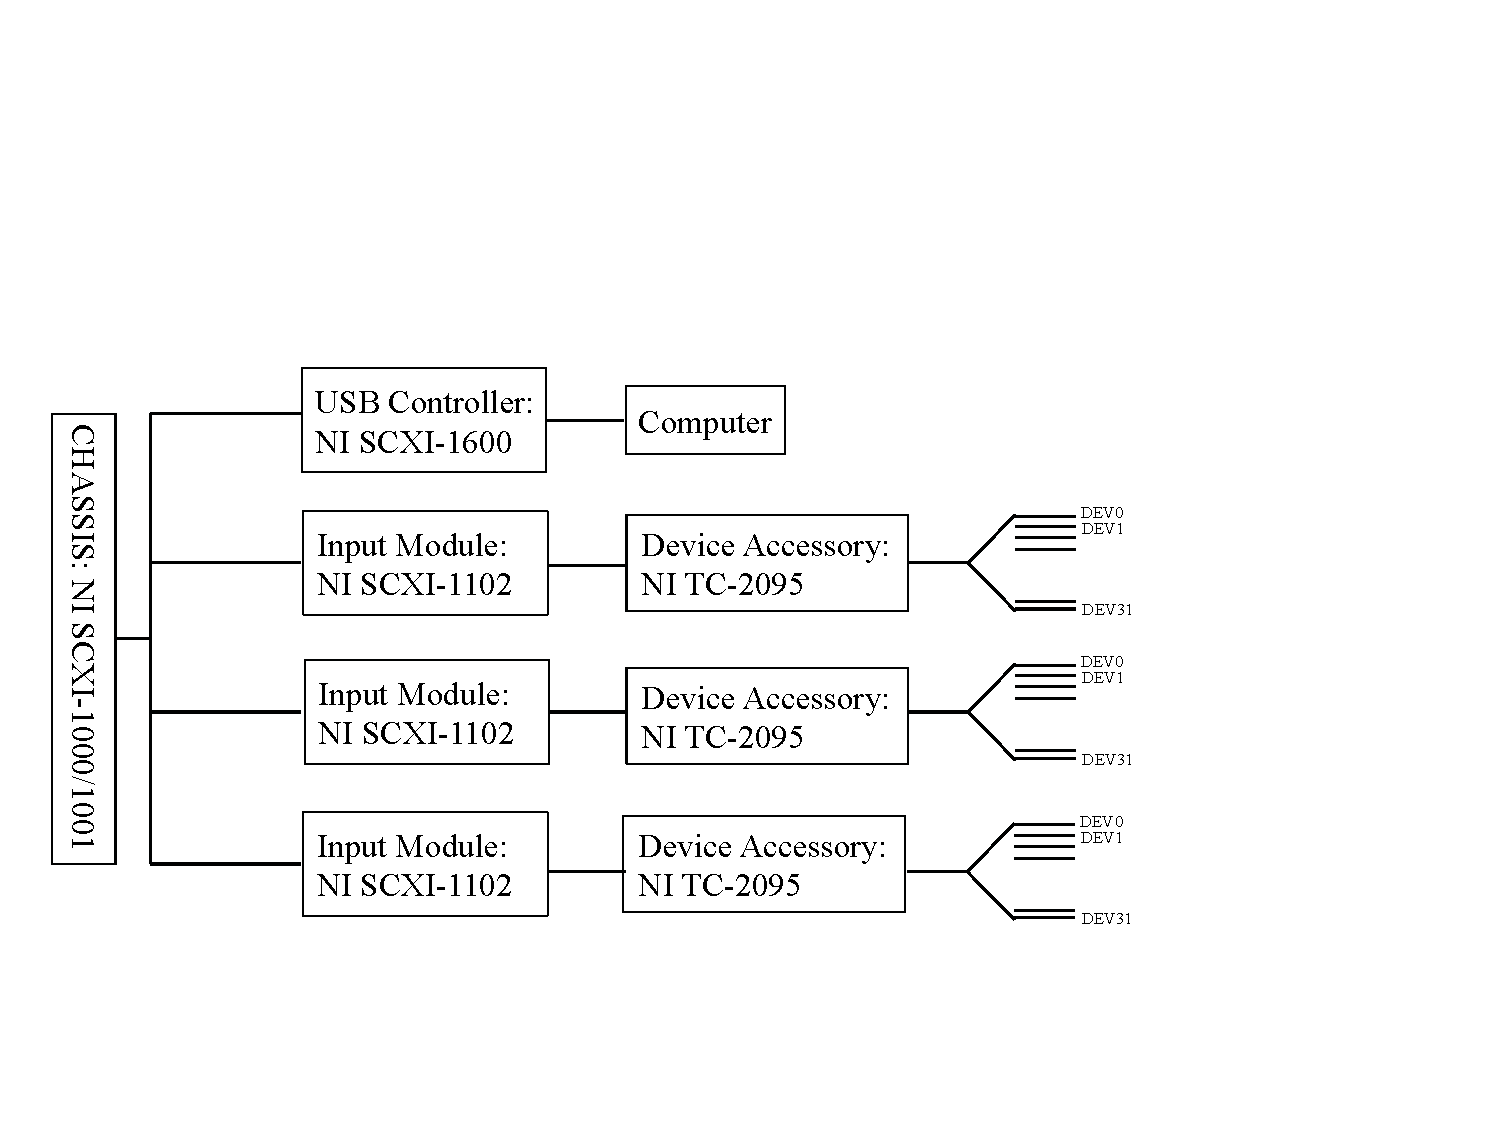
\includegraphics[width=5in]{Figures/DAQ_Schematic}
\caption{Schematic of data acquisition hardware.}
\label{fig:daq_schem}
\end{figure}

\section{Software}
Channel lists are built using NI-MAX and fed into 32-bit NI LabVIEW as a task using NI-DAQmx. Note that in the current configuration, the computer must also have a 32-bit operating system on it.

\chapter{Thermocouples}
\label{chap:thermocouple}

Two types of type~K thermocouples (TCs) are used: bare bead and metal sheathed. The bare bead TCs are made from 30~gauge glass braid insulated solid wire. The bare bead thermocouples are used in the TC trees and single point measurements. The metal sheathed TCs (\#125-KSL-600-U from Furnace Parts) have a 1/8~in diameter Inconel 600 sheath and an ungrounded junction. These TCs are moisture proof and are typically used in conjunction with bi-directional probes. The sheathed TCs are typically ordered with a 48~in TC and 120~in type~K lead wire (NIST01A from Furnace Parts) or a 144~in TC and 120~in type K lead wire (NIST01B from Furnace Parts).

\section{Uncertainty}

\begin{table}[h!]
\centering
\captionof{table}{Thermocouple Uncertainty}\label{tab:TC_uncertain}
\begin{tabular}{lll}
\toprule[1.5pt]
Thermocouple Type  &  Temperature Range     &  Error                                      \\
\midrule
Bare bead (SLE)    &  0 - 1250 $^{\circ}$C  &  MAX($\pm$ 1.1$^{\circ}$C; $\pm$ 0.4 $\%$)  \\
Inconel sheathed   &  0 - 1260 $^{\circ}$C  &  MAX($\pm$ 1.1$^{\circ}$C; $\pm$ 0.4 $\%$)  \\
\bottomrule[1.25pt]
\end{tabular}\par
\end{table}

\section{Thermocouple Welders}

Two different welders are used to construct the bare bead TCs. The Miyachi Unitek TC Welder (01-0196-02) is a manual feed thermocouple welder designed to weld thermocouple wires together without oxide layers by using argon cover gas. The welder can handle wires from 38~gauge to 20~gauge. 

\section{Thermocouple Extension Wire}

Two sets of type~K extension wire are used: single pair (EXPP-K-24-S-1000) or 20 pair (20KX24SPP). Both wires are 24~gauge, 7-32 stranded, polyvinyl coated wire.

\section{Thermocouple Connectors}

Thermocouple miniature connectors are high temperature liquid crystal polymer (HMPW-K-M/F). Thermocouple miniature panel jacks are used with the BDP boxes (MPJ-K-F).

\begin{table}[h!]
\centering
\captionof{table}{Thermocouple Connections}\label{tab:TC_connect}
\begin{tabular}{lll}
\toprule[1.5pt]
Use                & Connection End 1   & Connection End 2    \\
\midrule
TC Tree/Single TC  & TC Bead            &  Male               \\ 
Inconel sheathed   & TC Bead            &  Male               \\
Single Extension   & Female             &  Male               \\
BDP TC Extension   & Male               &  Male               \\
BDP Box            & Female Panel Jack  &  Female Panel Jack  \\
20 Pair Extension  & Female Panel Jack  &  Male               \\
\bottomrule[1.25pt]
\end{tabular}\par
\end{table}



\chapter{Bi-Directional Probes}
\label{chap:bdp}

Bi-directional probes are order from ... size specs. Pressure measurements are made using a XX Setra.

\begin{figure}[h!]
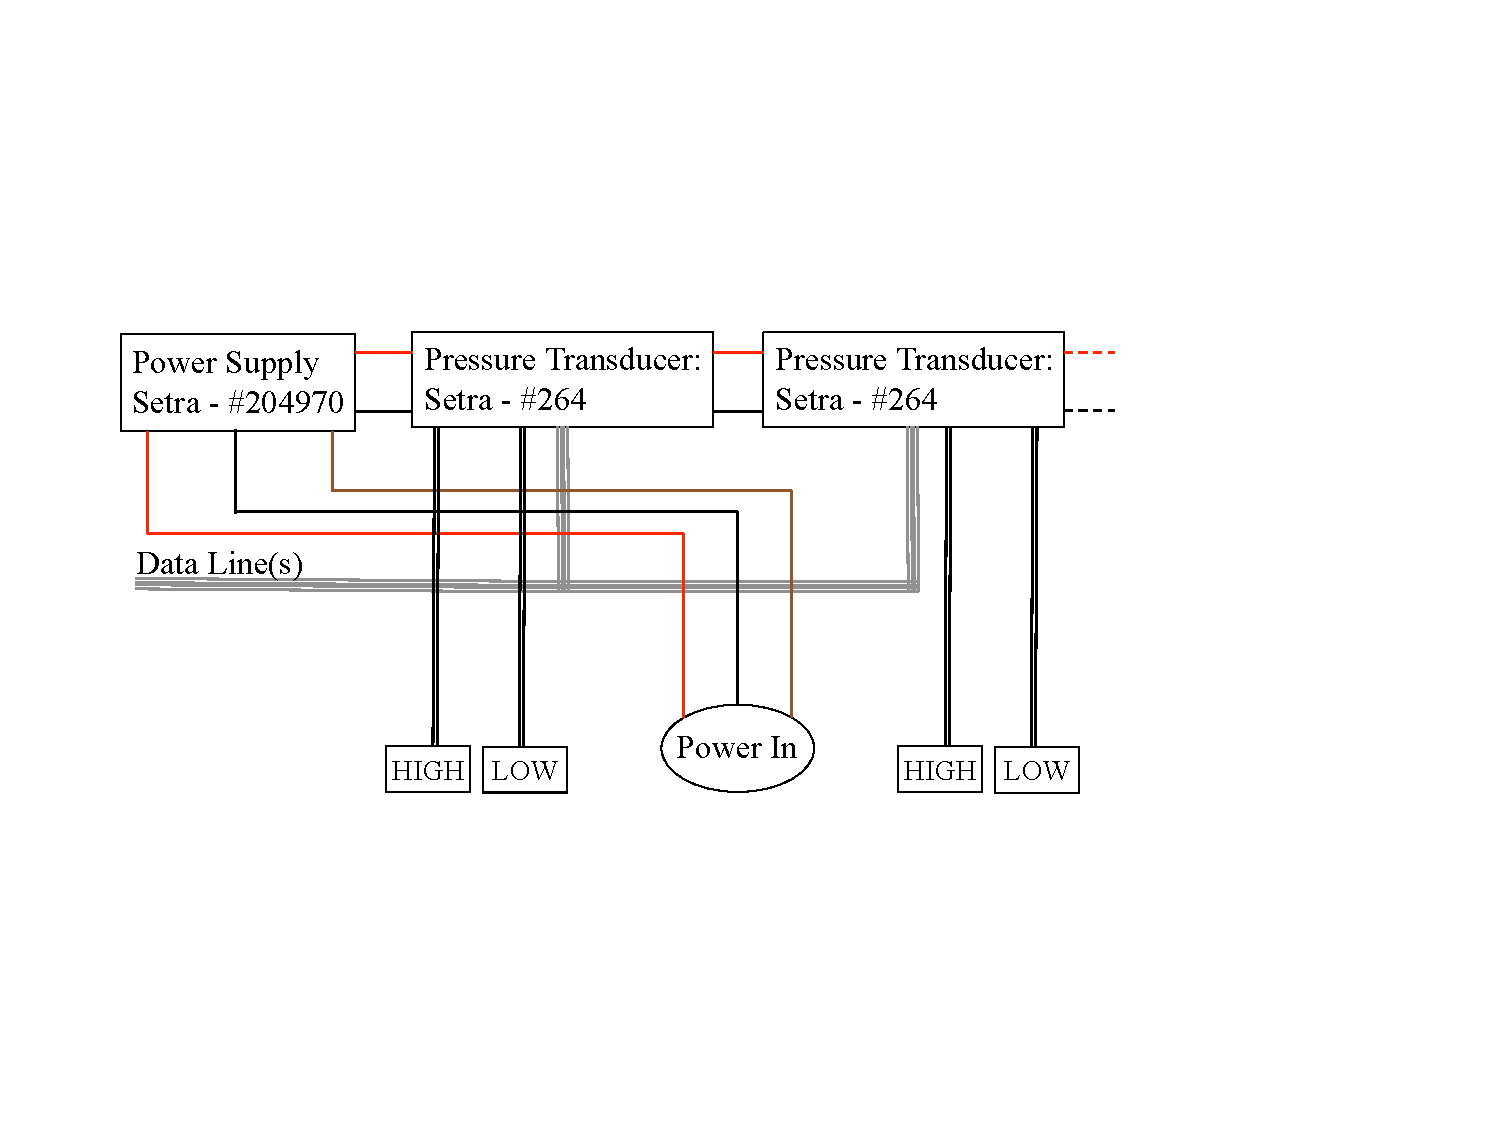
\includegraphics[width=5in]{Figures/BDP_Box}
\caption{Schematic of pressure measurement setup for use with BDPs.}
\label{fig:bdp_schem}
\end{figure}

\section{Uncertainty}

Uncertainty


\chapter{Heat Flux Gauges}

Medtherm Corporation Schmidt-Boelter total heat flux gages and radiometers are used with full scale outputs that range from 20 kW/m$^2$ to 100 kW/m$^2$. Each transducer outputs millivolts. Voltage is converted to heat flux using a conversion factor provided on each device's unique data sheet.

\section{Uncertainty}

Calibration is performed in compliance with ISO/IEC 17025, ANSI/NCSL Z540-1, and MIL-STD-45662A to Medtherm PI-20 with traceability to the National Institute of Standards and Technology. The total expanded uncertainty is $\pm 3\%$ with a coverage factor = 2 (95 $\%$ confidence level).


\chapter{Gas Analyzer}
\label{chap:Gas_Analyzer}

The CAI 602P Gas Analyzer can detect gas concentrations for CO$_2$, CO, and O$_2$ and output a voltage from 0~V to 5~V, which corresponds to 0~\% gas concentration to full-scale concentration.

\section{Internals}

The internal pump is located in the center of the chassis. The O$_2$ sensor is located under the foam cover. The CO sensor is located towards the front panel of the gas analyzer, and the CO$_2$ sensor is located towards the rear panel.

\section{Usage}

Important Note: The optimal pressure from the upstream sample and calibration gas is 0~psi! The internal gas analyzer components should never have an upstream pressure in excess of 2~psi. Pressures to the gas analyzer in excess of 2~psi may damage or dislodge the internal plumbing or pump diaphragms.

\begin{itemize}
\item Turn on the gas analyzers. The gas analyzers should warm up for about one hour before usage
\item Perform zero and span calibration on all analyzers.
    \begin{itemize}
    \item Flow N$_2$ and zero the CO$_2$, CO, and O$_2$ channels.
    \item Flow CO$_2$/CO calibration gas and span the CO$_2$ and CO channels.
    \item Use ambient air to span the O$_2$ channel.
    \end{itemize}
\item Set the upper ranges to the appropriate setting, which corresponds to 5~V on the output to the DAQ.
\item Measure the delay time for the sample gas to travel in the plumbing to the analyzer. You can do this by holding a CO$_2$ source near the sample port and measuring the time from exposing the sample port until the gas analyzer reads an increased value. Record this time so that the gas concentration can be offset later.
\item You are ready to record data to the DAQ.
\end{itemize}

\section{External Plumbing}

Calibration (span) gas (CO$_2$ and CO) $\rightarrow$ Bypass tee $\rightarrow$ Span gas inlet.

Sample tubes $\rightarrow$ Filter in dry ice (for scrubbing and cooling) $\rightarrow$ Sample pump (bypass value is on) $\rightarrow$ Sample inlet on gas analyzer $\rightarrow$ Outlet tube directed away from operator.

\section{Uncertainty}

Uncertainty

\section{Diagnostics}

\subsection{No Internal Flow}

If the flow drops to zero, then display the flow diagnostics by pressing Main $\rightarrow$ F3. Check the internal flow value for the three gases. If it is zero, then there might be a issue with the internal plumbing if the upstream pressure (from sample or calibration gases) exceeded 2~psi. Check power to the internal pump and ensure that it is operating.

\subsection{Bad Gas Concentration Readings}

If the channel is reading gas concentration values out of range or sporadic values, you may need to clean the internal sensor cell windows. Check the raw voltages in the analyzer setup by pressing Main $\rightarrow$ F5 $\rightarrow$ F6 $\rightarrow$ F2, then cycle through each gas using the left/right arrows. The raw voltages should be around 1.0~V at 0~\% concentration, and 9~V at full-scale concentration. Refer to Section~10 of the CAI 600P User Manual for more information.

\subsection{Diagnostic Information}

The following screens provide useful diagnostic information that can be sent to technical support:
\begin{itemize}
\item To display the version and serial number, press Main $\rightarrow$ F5 $\rightarrow$ F10.
\item To display flow diagnostics, press Main $\rightarrow$ F3.
\item To display raw voltage/channel values, press Main $\rightarrow$ F5 $\rightarrow$ F6 $\rightarrow$ F2, then cycle through each gas using the left/right arrows.
\end{itemize}

Refer to Section~10 of the CAI 600P User Manual for more information on maintenance and troubleshooting.


\chapter{Video}
\label{chap:Video}

\section{Digital Video Recorder Notes}

Model number: Samsung SRD-1680D

Samsung Customer Service: 877-213-1222

When running the ``Backup'' operation (to export the DVR movies to an external HDD), the DVR splits up files into 2.08 GB .avi movie files. See the video editing workflow section for information on joining multiple split videos into a single video file.

\subsection*{FAQ}

\begin{itemize}
\item Can I dump .avi files directly to an external drive? Quality?
    \begin{itemize}
    \item Can dump directly to AVI for a given date/time range, retains 1080 HD quality
    \end{itemize}
\item How are hard disks formatted in DVR (FAT32, exFAT, proprietary)?
    \begin{itemize}
    \item NTFS formatted
    \end{itemize}
\item How are files stored internally (.avi, proprietary)?
    \begin{itemize}
    \item Saved internally in DVR format, can export to AVI or to SCC (proprietary format)
    \end{itemize}
\item Can the internal drives be configured as RAID?
    \begin{itemize}
    \item Not internally
    \end{itemize}
\item What happens if one drive fails and other internal drives are available while recording?
    \begin{itemize}
    \item Seamless failover to other available drives
    \end{itemize}
\item How should an external drive be formatted?
    \begin{itemize}
    \item External USB drive should be formatted as FAT32. You can do this using the built in format function.
    \end{itemize}
\item Limit on number of connected smartphone viewers or remote viewers?
    \begin{itemize}
    \item Remote: Search 3, Live unicast 10, Live multicast 20
    \item Mobile: 1 Live, 1 CH playback
    \end{itemize}
\end{itemize}

\section{Video Editing Workflow}

\subsection{Digital Video Recorder}

The process for recording and extracting video from the DVR is as follows:
\begin{enumerate}
\item Record video.
\item Backup the video to an external drive to .avi format (H.264 codec and AVI container).
\item Convert the .avi videos to .mp4 format (H.264 codec and MPEG-4 container) for editing. A tool such as Handbrake is recommended.
\end{enumerate}
It is recommended that you maintain the original .avi files and subtitle files, which contain the date/timestamp information for future reference.

\subsection{Combining Videos}

The GoPro cameras and DVR split long videos into multiple files because of the format of the file systems that they write to. If you need to combine multiple .mp4 videos into one file, you can use a tool such as MP4Box or Avidemux. The benefit of these tools over a full video editor is that they can perform simple video operations without reencoding the video, so the processing is much faster. 

Multiple video files can also result from the DVR if a video channel temporarily loses signal. If this is the case, be sure to add blank video to pad any time that passed while the video channel signal was lost.

For example, to seamlessly combine two video files (video\_1.mp4 and video\_2.mp4) into one video file (video\_output.mp4), the command line tool MP4Box can be used with the following command

\begin{verbatim}
MP4Box -cat video_1.mp4 -cat video_2.mp4 -new video_output.mp4
\end{verbatim}

\subsection{Splitting Videos}

You can split an .mp4 video into multiple videos (without reencoding) with MP4Box. For example, if you have a 60~s video (video\_input.mp4), you can extract video from 30~s to 60~s and save the output to a new file (video\_output.mp4) with the following command

\begin{verbatim}
MP4Box -splitx 30:60 video_input.mp4 -out video_output.mp4
\end{verbatim}

\subsection{Creating Multi-Camera Videos}

You can combine multiple videos into a multi-camera video using software such as Adobe Premiere Pro or any other non-linear video editing software.


\chapter{Water Flow Sensor}
\label{chap:Water_Flow_Sensor}

\section{Arduino Config, Setup, and Data Logging}

The Arduinos record voltage data locally, and they transmit voltage data to the host computer via the AMQP messaging protocol. The host computer uses RabbitMQ to act as a broker. Python scripts and the pika module send and receive AMQP messages. The following steps setup the host computer and Arduinos for this purpose.

\subsection{Host Computer (RabbitMQ)}

Note: the following assumes that the server/host computer's address is 192.168.1.100. It's best to configure the host computer with a static IP address using static DHCP or manually.

\begin{enumerate}
\item Install RabbitMQ for your platform and start the RabbitMQ server (./sbin/rabbitmq-server on Mac or Linux).
https://www.rabbitmq.com/
\item Copy the receive\_data.py script from the NIST-FIRE repository to the data logging computer.
\item Install Python (The Anaconda Python distribution from Continuum Analytics is recommended)
\item Install the pika module for Python using
\begin{verbatim}
pip install pika
\end{verbatim}
\item Run the receive\_data.py script as
\begin{verbatim}
python receive_data.py 192.168.1.100 output.csv
\end{verbatim}
\end{enumerate}

\subsection{Host Computer (NTP Time Server)}

On Windows, download and install the NTP server

http://www.meinbergglobal.com/english/sw/ntp.htm

Note: you might need to disable the Windows Firewall service so that incoming connections will not be blocked.

Mac and Linux use NTP natively.

\subsection{Arduino Client (Sketch)}

\begin{enumerate}
\item Install Arduino IDE
http://arduino.cc/
\item Plug the Arduino Yun into the USB port of the host computer.
\item Set the Tools > Board to Arduino Yun and the Tools > Port to the /dev/ttyusbmodemXXXXXX setting that matches the plugged-in Arduino.
\item A Sketch is a script that runs on the Arduino microcontroller. Using the Arduino IDE, install the adc\_voltage Sketch on the Arduino from the NIST-FIRE repository. This enables the reading and writing of data from the analog-to-digital converter via the REST API on the Arduino. Note: this sketch requires the Adafruit ADS 1X15 library from https://github.com/adafruit/Adafruit\_ADS1X15.
\end{enumerate}

\subsection{Arduino Client (Linux)}

\begin{enumerate}
\item Unplug the Arduino from the computer, and power on the Arduino from the battery.
\item Connect to the Arduino WiFi network. Access the Arduino web interface (http://arduino.local) with the default password of ``arduino''. Set the Arduino name (referred to as <arduino\_name> in the following steps), time zone, and WiFi network information on the Arduino web config. Also, set the ``REST API Access'' to be ``Open''.
\item SSH to the Arduino at root@<arduino\_name>.local and install the SFTP server, ntpclient, pip, and pika (for AMQP) on the Arduino
\begin{verbatim}
opkg update
opkg install openssh-sftp-server ntpclient distribute python-openssl
easy_install pip
pip install pika
\end{verbatim}
\item By default, the microSD card on the Arduino is mounted at /mnt/sda1. Copy the send\_data.py script from the NIST-FIRE repository to /mnt/sda1 on the Arduino.
\item Go to System > Startup > Local Startup in the Arduino web config and add a startup line to the Local Config section (/etc/rc.local)
\small
\begin{verbatim}
python /mnt/sda1/send_data.py 192.168.1.100 <arduino_name> /mnt/sda1/output.csv
\end{verbatim}
\normalsize
\clearpage
\item The default NTP service is not very robust, so we will replace it with ntpclient and have it sync with the NTP server every 2 minutes. Disable the default NTP service using
\begin{verbatim}
/etc/init.d/sysntpd disable
\end{verbatim}
Configure the ntpclient service by editing /etc/config/ntpclient to be
\begin{verbatim}
config ntpserver
        option hostname '192.168.1.100'
        option port     '123'

config ntpserver
        option hostname '0.pool.ntp.org'
        option port     '123'

config ntpserver
        option hostname '1.pool.ntp.org'
        option port     '123'

config ntpserver
        option hostname '2.pool.ntp.org'
        option port     '123'

config ntpserver
        option hostname '3.pool.ntp.org'
        option port     '123'

config ntpdrift                                 
        option freq     '0'                     
                                                
config ntpclient                                
        option interval 120
\end{verbatim}
\item Reset power to the Arduino, and then it should start broadcasting data values within about 2 minutes of booting.
\end{enumerate}

\section{Parts}

\begin{itemize}
\item Mouser \#:   517-929834-02-36-RK \\
Mfr. \#: 929834-02-36-RK \\
Desc.: Headers \& Wire Housings FULL STICK HDR/36POS \\
\$1.13

\item Mouser \#:   932-MIKROE-197 \\
Mfr. \#: MIKROE-197 \\
Desc.:  Daughter Cards \& OEM Boards SMARTPROTO PROTO ADAPTER BOARD \\
\$4.90
\end{itemize}


%  ==============
%  = Appendices =
%  ==============


\appendix

\chapter{Testing Procedure}

\section{Initial Startup}

\begin{itemize}
\item Power on the following devices:
    \begin{itemize}
    \item Uninterruptible Power Supplies (UPSs)
    \item WiFi routers
    \item Hose flow / Arduino laptop with NTP, RabbitMQ, Python receive\_data.py script
    \item DAQs and laptops
    \item Gas analyzers (leave running as long as possible during testing)
    \item Digital video recorder (DVR)
    \item Bullet cameras
    \item Thermal imaging cameras (TICs) (check battery level)
    \item Digital video cassette recorders (DVCRs) (check battery level)
    \item GoPros (check battery level)
    \item Video cameras (check battery level)
    \end{itemize}
\end{itemize}

\section{Calibration}

\begin{itemize}
\item Synchronize time on DAQ computers and digital video recorder

\item Verify operation of all:
    \begin{itemize}
    \item Video channels
    \item DAQ channels
    \item Check toggle switches on TC-2095s for appropriate measurement device
    \item Gas analyzers
    \end{itemize}

\item Calibrate gas analyzers with zero and span gases

\item 1 minute calibration run to separate output file (cover BDPs, check TCs, etc.)

\end{itemize}

\section{Primary Testing Procedure}

\begin{itemize}
\item Verify testing procedure with all personnel
\item Safety checks

\item Power on gas analyzer pump

\item Turn on water for heat flux gauges

\item Check Arduino battery level
\item Power on Arduino data loggers

\item Start recording on:
    \begin{itemize}
    \item GoPros
    \item Video cameras
    \item DVCRs (Mobile TIC)
    \end{itemize}

\item Start synced recording on: [MARK DATE/TIME]
    \begin{itemize}
    \item DVR
    \item DAQ data
    \end{itemize}

\item 1 minute pre-test run (with all doors closed)

\item Begin test [MARK DATE/TIME]

\item Follow testing procedure

\item End test [MARK DATE/TIME]

\item Stop synced recording on: [MARK DATE/TIME]
    \begin{itemize}
    \item DAQ
    \item DVR
    \end{itemize}

\item Stop recording on:
    \begin{itemize}
    \item GoPros
    \item Video cameras
    \item DVCRs (Mobile TIC)
    \end{itemize}

\item Power off gas analyzer pump

\item Power off Arduino data loggers

\item Verify successful recording and operation of all DAQ channels in output file

\item Prepare for next test
\end{itemize}

\section{Data Dump}

\begin{itemize}
\item Retrieve data from:
    \begin{itemize}
    \item DAQ
    \item DVR
    \item GoPros
    \item Video cameras with digital media
    \item Arduinos
    \end{itemize}

\item Swap and label tapes from video cameras and DVCRs as needed

\item Make 3 copies of all data on external hard drives

\item Verify integrity of data

\item On return from trip, extract video from DVCRs
\end{itemize}

\section{Battery Charging}

\begin{itemize}
\item Charge all batteries on:
    \begin{itemize}
    \item Laptops
    \item Arduinos
    \item Bullet camera batteries
    \item TICs
    \item GoPros
    \item Video cameras
    \item DVCRs
    \item Radios
    \end{itemize}
\end{itemize}


\end{document}
